\section{WS 1.3 - 9 - MAT - Eishockeytore - OA - Matura HT 2015/16}

\begin{beispiel}[WS 1.3]{1} %PUNKTE DES BEISPIELS
In der österreichischen Eishockeyliga werden die Ergebnisse aller Spiele statistisch ausgewertet. In der Saison 2012/13 wurde über einen bestimmten Zeitraum erfasst, in wie vielen Spielen jeweils eine bestimmte Anzahl an Toren erzielt wurde. Das nachstehende Säulendiagramm stellt das Ergebnis dieser Auswertung dar.


\begin{center}
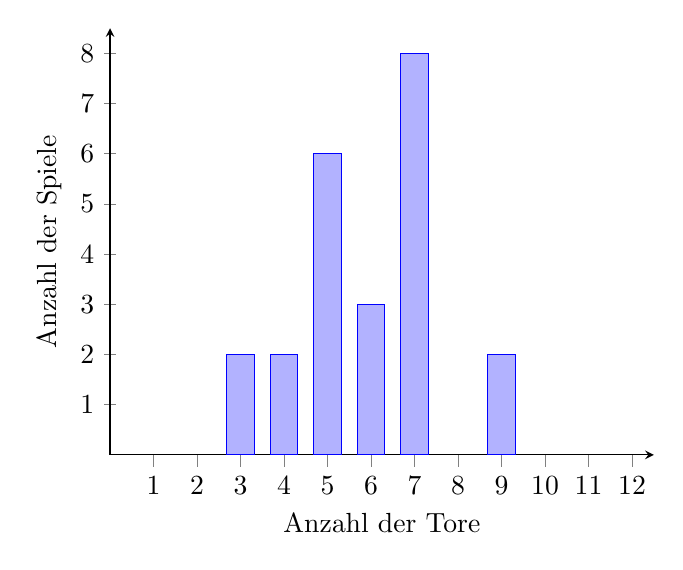
\begin{tikzpicture}
  \begin{axis}[/pgf/number format/1000 sep={},axis lines=left,
	grid=none, y grid style={line width=.001pt,draw=white}, ybar,xmin=0,xmax=12.5,ymin=0, ymax=8.5, xlabel= Anzahl der Tore, ylabel= Anzahl der Spiele, ytick={1,2,3,4,5,6,7,8}, xtick={1,2,3,4,5,6,7,8,9,10,11,12},
    width=0.7\textwidth, height=7cm]
    \addplot coordinates {(3,2) (4,2) (5,6) (6,3) (7,8) (9,2)};
  \end{axis}
\end{tikzpicture}
\end{center}


Bestimme den Median der Datenliste, die dem Säulendiagramm zugrunde liegt.

\antwort{Der Median der Datenliste ist 6.}

\end{beispiel}